% Created 2020-07-23 jue 11:50
% Intended LaTeX compiler: pdflatex
\documentclass[presentation,aspectratio=1610]{beamer}
\usepackage[utf8]{inputenc}
\usepackage[T1]{fontenc}
\usepackage{graphicx}
\usepackage{grffile}
\usepackage{longtable}
\usepackage{wrapfig}
\usepackage{rotating}
\usepackage[normalem]{ulem}
\usepackage{amsmath}
\usepackage{textcomp}
\usepackage{amssymb}
\usepackage{capt-of}
\usepackage{hyperref}
\usepackage{khpreamble, euscript}
\DeclareMathOperator{\atantwo}{atan2}
\newcommand*{\ctrb}{\EuScript{C}}
\newcommand*{\obsv}{\EuScript{O}}
\usetheme{default}
\author{Kjartan Halvorsen}
\date{\today}
\title{Control computarizado - Modelos en espacio de estados}
\hypersetup{
 pdfauthor={Kjartan Halvorsen},
 pdftitle={Control computarizado - Modelos en espacio de estados},
 pdfkeywords={},
 pdfsubject={},
 pdfcreator={Emacs 26.3 (Org mode 9.3.6)}, 
 pdflang={English}}
\begin{document}

\maketitle

\section{PMSM - Motor syncrono de Iman permanente}
\label{sec:org508c1e6}

\begin{frame}[label={sec:org4b4c1c2}]{PMSM - Motor síncrono de imán permanente}
\begin{center}
\includegraphics[width=0.9\linewidth]{../../figures/permanent-motor.jpg}
\end{center}
\end{frame}
\begin{frame}[label={sec:orga7496f7}]{PMSM - Motor síncrono de imán permanente}
\begin{center}
\includegraphics[width=0.9\linewidth]{../../figures/pmsm_control_block_diag.png}
\end{center}
\end{frame}

\begin{frame}[label={sec:org302e4a0}]{Modelo identificado}
\begin{center}
  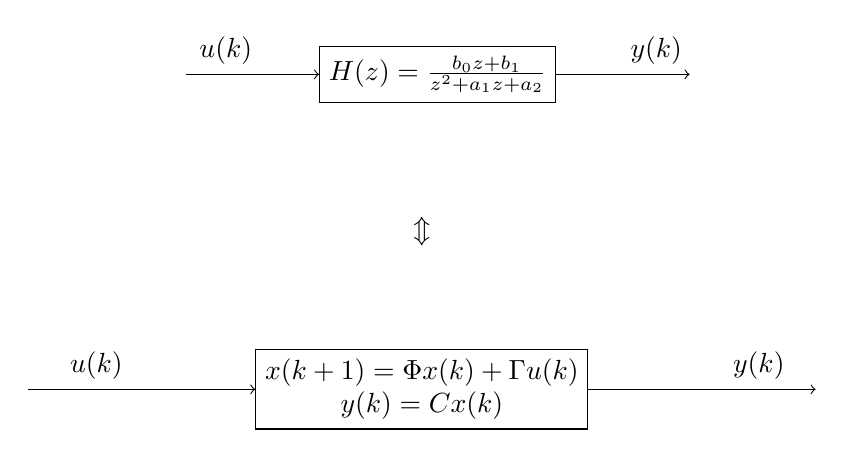
\begin{tikzpicture}[node distance=32mm, block/.style={rectangle, draw, minimum width=15mm}, sumnode/.style={circle, draw, inner sep=2pt}]

    \node[coordinate] (input) {};
    \node[block, right of=input] (plant)  {$H(z) = \frac{b_0z + b_1}{z^2 + a_1 z + a_2}$};
    \node[coordinate, right of=plant] (output) {};

    \draw[->] (input) -- node[above, pos=0.3] {$u(k)$} (plant);
    \draw[->] (plant) -- node[above, near end] {$y(k)$} (output);

    \begin{scope}[yshift=-2cm, xshift = 3cm]
    \node {$\Updownarrow$};
    \end{scope}

    \begin{scope}[yshift=-4cm, node distance=50mm, xshift=-2cm]
    \node[coordinate] (input) {};
    \node[block, right of=input, align=center] (plant)  {$x(k+1) = \Phi x(k) + \Gamma u(k)$\\$y(k) = C x(k)$};
    \node[coordinate, right of=plant] (output) {};

    \draw[->] (input) -- node[above, pos=0.3] {$u(k)$} (plant);
    \draw[->] (plant) -- node[above, near end] {$y(k)$} (output);
    \end{scope}



  \end{tikzpicture}
\end{center}
\end{frame}

\begin{frame}[label={sec:orgc9047ad}]{Formas canónicas}
Dado función de transferencia 
\[ H(z) = \frac{b_1 z^2 + b_2 z + b_3}{z^3 + a_1z^2 + a_2z + a_3}.\] 
Encuentra una representación en espacio de estados.
\begin{align*}
 x(k+1) &= \Phi x(k) + \Gamma u(k) \\
 y(k) &= C x(k)
 \end{align*}

\begin{itemize}
\item Forma canónica de control
\item Forma canónica de observador
\end{itemize}
\end{frame}

\begin{frame}[label={sec:orgaf260e0}]{Forma canónica de control}
Dado función de transferencia 
\[ H(z) = \frac{b_1 z^2 + b_2 z + b_3}{z^3 + a_1z^2 + a_2z + a_3}.\] 

\begin{align*}
 x(k+1) &= \begin{bmatrix} -a_1 & -a_2 & -a_3\\1 & 0 & 0\\0 & 1 & 0\end{bmatrix} x(k) + \begin{bmatrix}1\\0\\0\end{bmatrix} u(k) \\
 y(k) &= \begin{bmatrix} b_1 & b_2 & b_3 \end{bmatrix} x(k)
 \end{align*}
\end{frame}


\begin{frame}[label={sec:org21996c0}]{Forma canónica de observador}
Dado función de transferencia 
\[ H(z) = \frac{b_1 z^2 + b_2 z + b_3}{z^3 + a_1z^2 + a_2z + a_3}.\] 

\begin{align*}
 x(k+1) &= \begin{bmatrix} -a_1 & 1 & 0\\-a_2 & 0 & 1\\-a_3 & 0 & 0\end{bmatrix} x(k) + \begin{bmatrix}b_1\\b_2\\b_3\end{bmatrix} u(k) \\
 y(k) &= \begin{bmatrix} 1 & 0 & 0 \end{bmatrix} x(k)
 \end{align*}
\end{frame}


\begin{frame}[label={sec:org3ea89d0}]{Formas canónicas - ejercicio}
\alert{Actividad} Encuentra las formas canónicas de control y de observador para la función de transferencia del motor
\[H(z) = \frac{23.3z - 6.9}{z^2 - 1.40z + 0.61}\]
\end{frame}



\section{Apollo moon lander}
\label{sec:org9aef93b}
\begin{frame}[label={sec:org3a0c0db}]{Modelación}
\end{frame}
\begin{frame}[label={sec:orgbb713d6}]{Ejemplo - El módulo lunar de Apollo}
\begin{center}
\includegraphics[width=\linewidth]{fig-apollo}
\end{center}
\end{frame}
\begin{frame}[label={sec:orgf920e21}]{Ejemplo - El módulo lunar de Apollo}
\begin{center}
\includegraphics[width=0.8\linewidth]{fig-apollo}
\end{center}
\alert{Actividad} ¿Cuál es la función de transferencia del sistema?
\[1: \; G(s) = \frac{k_1 k_2}{s^2}\qquad 2: \; G(s) = \frac{k_1 k_2}{s(s^2 + 1)} \qquad 3: \; G(s) = \frac{k_1 k_2}{s^3}\]
\end{frame}

\begin{frame}[label={sec:orgd5dbd7f}]{Ejemplo - El módulo lunar de Apollo}
\begin{center}
\includegraphics[width=0.8\linewidth]{fig-apollo}
\end{center}
\alert{Actividad} ¿Que sensores relevantes se puede usar para el control?
\end{frame}

\begin{frame}[label={sec:orgd8e1e4b}]{Ejemplo - El módulo lunar de Apollo}
\begin{center}
\includegraphics[width=0.7\linewidth]{fig-apollo}
\end{center}

Variables del estado: \(x = \begin{bmatrix} x_1 & x_2 & x_3 \end{bmatrix}^T = \begin{bmatrix} \dot{\theta} & \theta & \dot{z} \end{bmatrix}^T\). Con dinamica
\[ \begin{cases} \dot{x}_1 =  \ddot{\theta} = k_1 u\\ \dot{x}_2 = \dot{\theta} = x_1\\ \dot{x}_3 = \ddot{z} = k_2\theta = k_2x_2 \end{cases} \]
\end{frame}

\begin{frame}[label={sec:orgbf963a5}]{Ejemplo - El módulo lunar de Apollo}
Variables del estado: \(x = \begin{bmatrix} x_1 & x_2 & x_3 \end{bmatrix}^T = \begin{bmatrix} \dot{\theta} & \theta & \dot{z} \end{bmatrix}^T\). Con dinamica
\[ \begin{cases} \dot{x}_1 =  \ddot{\theta} = k_1 u\\ \dot{x}_2 = \dot{\theta} = x_1\\ \dot{x}_3 = \ddot{z} = k_2\theta = k_2x_2 \end{cases} \]

\alert{Actividad} Llena los matrices y vectores en el modelo de espacio de estados

\[ \dot{x} = \begin{bmatrix} \dot{x}_1\\\dot{x}_2\\\dot{x}_3\end{bmatrix} = \underbrace{\begin{bmatrix} \quad & \quad &\quad \\\quad & \quad& \quad\\ \quad& \quad &\quad \end{bmatrix}}_{A} \begin{bmatrix} x_1\\x_2\\x_3\end{bmatrix} + \underbrace{\begin{bmatrix} \quad \\ \quad \\\quad  \end{bmatrix}}_{B} u \]
\end{frame}


\begin{frame}[label={sec:orge11cccf}]{Modelación - ejercicio}
\begin{columns}
\begin{column}{0.5\columnwidth}
\includegraphics[height=0.5\textheight]{../../figures/mass-spring-damper}
\end{column}

\begin{column}{0.5\columnwidth}
 Queremos controlar la posición vertical \(X\) de una masa, aplicando una fuerza \(u\) en esta. En la posición relajada, \(X=0, \; \dot{X} =0\), la fuerza en el resorte es igual a la fuerza de gravedad.  
\[ m\ddot{X} = -kX - f\dot{X} + u\]
\alert{Actividad} Encuentra una representación del sistema en espacio de estados. 

\begin{align*}
\dot{x} &= A x + Bu\\ y &= Cx 
\end{align*}
\end{column}
\end{columns}
\end{frame}
\end{document}